\chapter{\heiti 调用接口程序}
\section{Python \heiti{接口程序}}
我司为用户提供了Python接口程序。用户可调用接口程序中的函数自己编程生成方波序列,并将其下载到硬件中,然后通过调用函数控制仪器播放自定义的方波序列。使用Python接口程序中的函数时可以参考我司为用户提供的“DDR3\_USB\_8chn\_Continue\_counter.py”文件中的调用方式。现将用户所需的函数列出,并加以解释。注意在调用接口程序中的函数时,定义的单个方波序列高低电平时间必须在7.5 ns 至2.6 s 之间,且必须是0.05 ns的整数倍。
\vspace{0.4cm}

\noindent\fontsize{12pt}{\baselineskip}\textbf{\heiti{函数}PB\_type\_program(pulse)}

传入参数“pulse”是一个列表(list\_0),列表中的每个元素仍然是一个列表(list\_1),每个list\_1均形如[`01010101', 0, 0, 20.0]。list\_1中的第一个元素为一个字符串,字符串由8个‘0’或‘1’组成,从左往右依次代表8个输出通道,‘0’代表该通道输出低电平,‘1’代表该通道输出高电平。list\_1中的第二和第三个元素没有意义,为0即可。list\_1中的第四个元素代表该方波序列状态的持续时间,单位为纳秒。例如用户想要在OUT1通道输出一个高电平时间长度为60 ns低电平时间为40.05 ns的方波序列,则用户可以令pulse=[[`10000000',0,0,60], [`00000000',0,0,40.05]],然后调用PB\_type\_program(pulse)即可将该方波序列下载到硬件中。
\vspace{0.4cm}

%\newpage
\noindent\fontsize{12pt}{\baselineskip}\textbf{\heiti{函数}start()}

函数没有传入参数,调用PB\_type\_program( )与Counter\_program( )后,再调用start( )即可向硬件发送指令使仪器开始播放方波序列。
\vspace{0.4cm}

\noindent\fontsize{12pt}{\baselineskip}\textbf{\heiti{函数}stop()}

此函数没有传入参数,用来向硬件发送指令,使仪器停止播放方波。在调用stop( )之后再次调用start( ),可以重新使仪器播放用户自定义的方波序列。
\vspace{0.4cm}

\noindent\fontsize{12pt}{\baselineskip}\textbf{\heiti{完整调用过程举例}}

pulse = [[`10000000',0,0,60],[`00000000',0,0,40.05]]\qquad  \#  定义方波序列

PB\_type\_program(pulse)\qquad            \#  下载方波序列

start( )\qquad          \#  开始播放方波序列

stop( )\qquad     \#  停止播放方波序列,仅在需要停止播放序列时使用

\section{C\heiti 接口程序}
我司为用户提供了C接口程序。用户可调用接口程序中的函数自己编程生成方波序列,并将其下载到硬件中然后控制仪器播放生成的方波序列。现将用户所需的函数列出,并作出解释。注意在调用接口程序中的函数时,定义的单个方波序列高低电平时间必须在7.5 ns至2.6 s之间,且必须是0.05 ns的整数倍。

%\newpage
\vspace{0.4cm}
\noindent\fontsize{12pt}{\baselineskip}\textbf{\heiti{函数}asg\_program\_all(char **flags,double *time\_length,unsigned long cmd\_num,\\unsigned char **buf,int *buf\_length)}
%\vspace{0.4cm}
\begin{table}[H]
%\begin{table}[!htbp]
\normalsize
%\caption{}
%\rowcolors{2}{gray!10}{gray!10}
\begin{tabular}{|m{7cm}<{\centering}|m{7cm}|}
%\begin{tabular}{p{0.5\textwidth}|p{0.5\textwidth}}
\rowcolor{blue!50}
\hline
传入参数 & \makebox[7cm][c]{参数描述} \\ \hline
char **flags & 参数“flags”是一个二维数组,每个元素均为形如“01011010”的字符串。字符串个数代表方波数据的个数,字符串中的‘0’或‘1’从左往右依次代表8个方波输出通道的的状态。‘0’ 代表低电平,‘1’ 代表高电平。\\ \hline
double *time\_length & 参数“time\_length”是一个double型一维数组。每个元素代表相应每个方波序列状态的时间长度,单位为纳秒。该数组长度必须与“flags”的数组长度相同。 \\\hline
unsigned long cmd\_num & 参数“cmd\_num”是一个正整数,表示方波序列数据的个数。 \\\hline
unsigned char **buf & 参数“buf”是一个二维空字符数组。即每个元素为一空字符串,字符串的个数为8,每个字符串的长为cmd\_num的10倍。 \\\hline
int *buf\_length & 参数“buf\_length”必须是\{0,0,0,0,0,0,0,0\}。 \\\hline
\end{tabular}
\end{table}

%\vspace{0.4cm}
\noindent\fontsize{12pt}{\baselineskip}\textbf{\heiti{函数}asg\_start( )}

此函数无传入参数,调用asg\_program\_all( )后,再调用asg\_start( )即可向硬件发送指令使仪器开始播放方波序列。

%\newpage
\vspace{0.4cm}
\noindent\fontsize{12pt}{\baselineskip}\textbf{\heiti{函数}asg\_stop( )}

 此函数无传入参数,用来向硬件发送指令,使仪器停止播放方波。在调用asg\_stop( )之后再次调用asg\_start( )可以重新使仪器播放方波序列。

%\vspace{0.6cm}
\newpage
\section{\heiti 两种接口程序比较}

现将Python接口程序与C接口程序中用户需要调用的函数做一对比,方便用户更好的理解调用接口程序的过程。
\begin{table}[H]
\normalsize
%\caption{}
%\rowcolors{2}{gray!10}{gray!10}
\begin{tabular}{|m{1.5cm}<{\centering}|m{5cm}<{\centering}|m{6.5cm}|}
\rowcolor{blue!50}
\hline
接口程序 & \makebox[6.6cm][l]{\qquad\qquad\qquad Python} & \makebox[6.0cm][c]{C}\\ \hline
\vspace{-0.4cm}\multirow{4}{1in}{\hspace{0.15cm} 函数名} & PB\_type\_program(pulse)将方波数据下载到硬件中。& asg\_program\_all(char **flags, double *time\_length, unsigned long cmd\_num, unsigned char **buf, int *buf\_length)用来将方波数据下载到硬件中。\\\cline{2-3}
&start( )开始播放方波序列。& asg\_start( )开始播放方波序列。\\\cline{2-3}
&stop( )停止播放方波序列。& asg\_stop( )停止播放方波序列。\\
\hline
\end{tabular}
\end{table}
%\begin{figure}
%\centering
%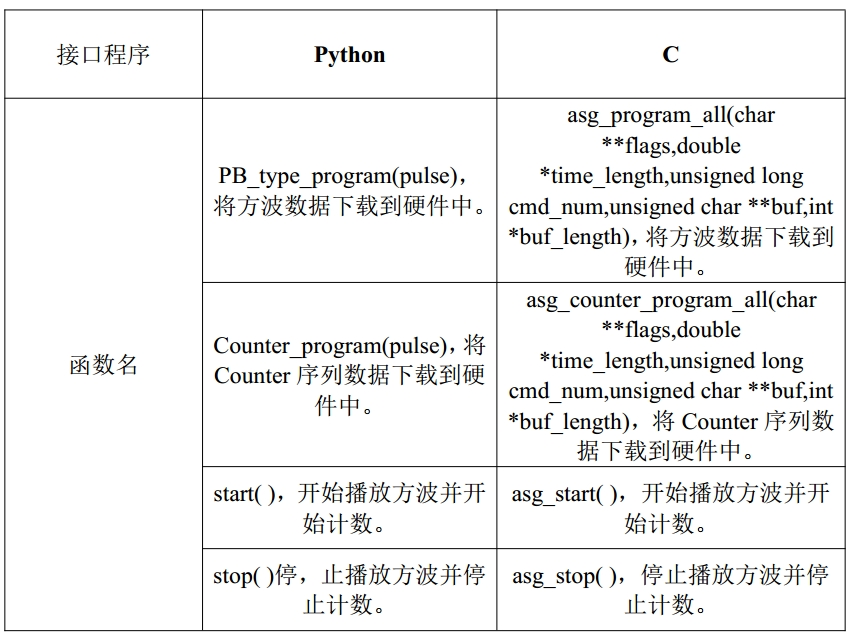
\includegraphics[width=16cm]{last_table}
%\end{figure}
